\section{Results}\label{sec:MLresults}
We first describe the calculated fuel consumption, before presenting the results of our hybrid machine learning approach, including a comparison of different machine learning algorithms using both the training set and the test set.
% Compare engineering estimates to reported values
%  - give mean and sd of calculated
%  - histogram or two-way
%  - compare to what IMO gets (fig 104)

Summary statistics for the annual fuel consumption, calculated as per \autoref{subsec:engcalc} are presented in \autoref{tab:calstats}. Over all three years of data, the mean calculated fuel consumption of 1407 tonnes is slightly higher than the reported average of 1343 tonnes. \autoref{fig:twoway_cal} presents the calculated versus reported values for both the training and test sets. For the training set, the \ac{R2} is only 0.275, which highlights the opportunity for improving the accuracy of fuel consumption and emissions estimates from the calculation-based approach.
% Source: ML_FC_..._train.csv
% TODO: check and adjust R^2 for calc on test

\begin{table}
    \centering
    % \begin{adjustbox}{max width=\textwidth}
    \begin{threeparttable}
        \caption{Calculated fuel consumption summary statistics}
        \label{tab:calstats}
        
\begin{tabular}[t]{>{\centering\arraybackslash}p{4em}>{\raggedleft\arraybackslash}p{3em}>{\raggedleft\arraybackslash}p{3em}>{\raggedleft\arraybackslash}p{3em}}
\toprule
\multicolumn{1}{>{\centering\arraybackslash}p{4em}}{Year} & \multicolumn{1}{>{\centering\arraybackslash}p{3em}}{count} & \multicolumn{1}{>{\centering\arraybackslash}p{3em}}{mean} & \multicolumn{1}{>{\centering\arraybackslash}p{3em}}{sd}\\
\midrule
2019 & 585 & 1440 & 1219\\
2020 & 671 & 1402 & 1292\\
2021 & 692 & 1383 & 1135\\
\bottomrule
\end{tabular}

        % \begin{tablenotes}[flushleft]\small
            % \item \textit{Note:} MAE is mean absolute error, and $R^2$ is the coefficient of determination. The best score for each metric is highlighted in bold.
        % \end{tablenotes}
    \end{threeparttable}
    % \end{adjustbox}
\end{table}

\begin{figure}
    \centering
    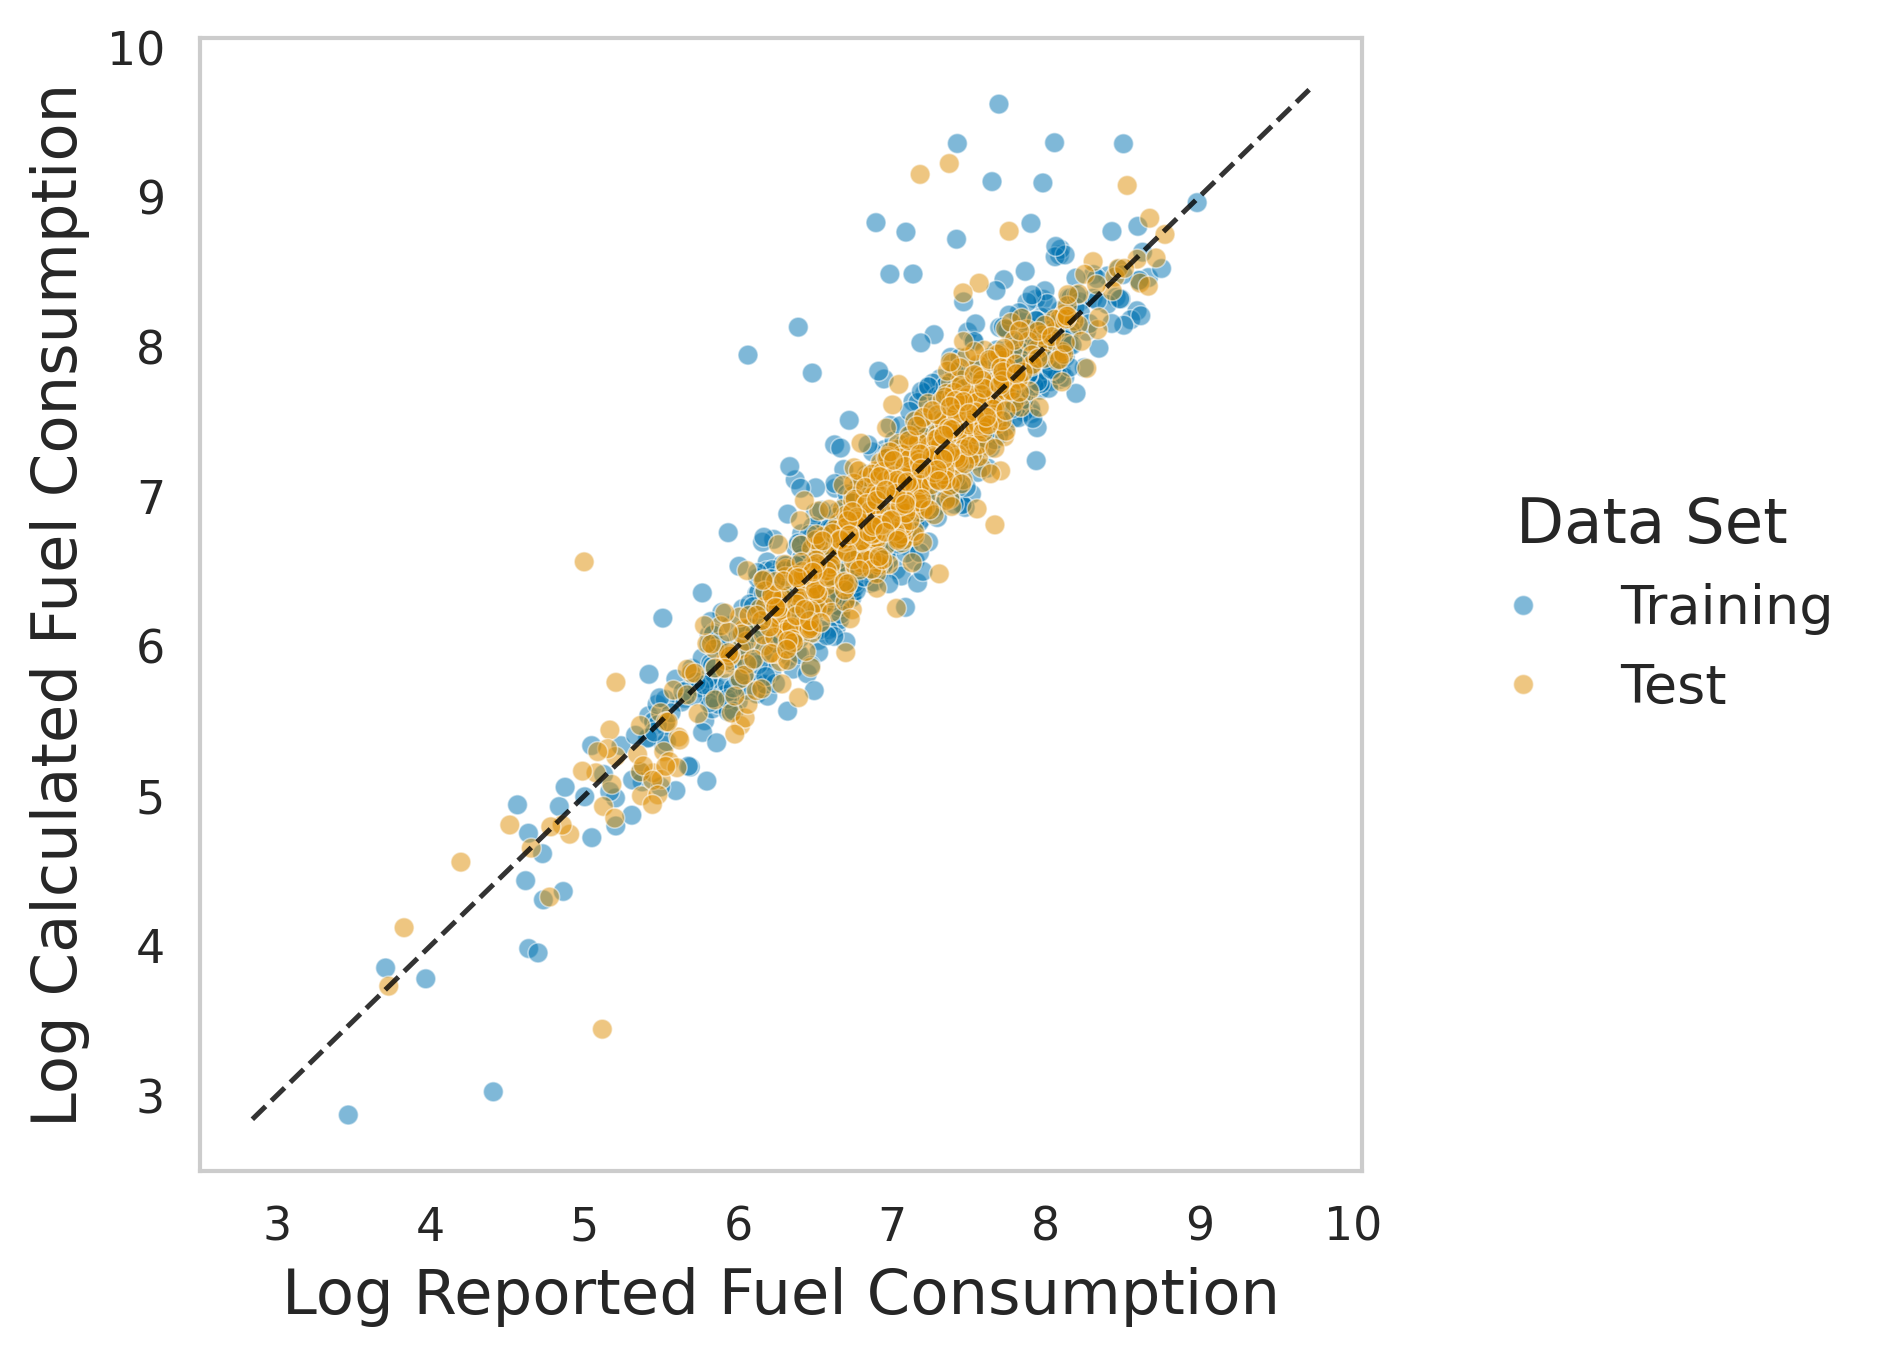
\includegraphics[width=0.65\textwidth]{ML_FC_Fm5dd_twoway_fc_filtered_traintest.png}
    \caption{Engineering calculations vs. reported fuel consumption}
    \label{fig:twoway_cal}
\end{figure}

% Tuning
The cross-validation training set performance of each optimally-tuned model is summarized in \autoref{tab:trainscores}, and the optimal parameters are provided in \autoref{tab:trainparams} in \autoref{app:ML}. The linear estimators perform slightly better than the tree-based models, both in terms of better average accuracy and less variation. Within the linear models, performance is almost identical, despite the regularization parameter being equal to one for ridge regression.
The overall best performance is achieved with ridge regression, giving an \ac{R2} of 0.956 and an \ac{MAPE} of 9.8\%. 

% Training set evaluation
\begin{table}
    \centering
    \begin{adjustbox}{max width=\textwidth}
    \begin{threeparttable}
        \caption{Training set cross-validation scores}
        \label{tab:trainscores}
        
\begin{tabular}[t]{lrrrrrr}
\toprule
\multicolumn{1}{c}{ } & \multicolumn{2}{c}{R$^2$} & \multicolumn{2}{c}{MAE (t)} & \multicolumn{2}{c}{MAPE (\%)} \\
\cmidrule(l{3pt}r{3pt}){2-3} \cmidrule(l{3pt}r{3pt}){4-5} \cmidrule(l{3pt}r{3pt}){6-7}
\multicolumn{1}{c}{Model} & \multicolumn{1}{c}{mean} & \multicolumn{1}{c}{sd} & \multicolumn{1}{c}{mean} & \multicolumn{1}{c}{sd} & \multicolumn{1}{c}{mean} & \multicolumn{1}{c}{sd}\\
\midrule
Ridge Regression & 0.956 & 0.019 & 122 & 13 & 9.8 & 0.7\\
Linear Regression & 0.956 & 0.020 & 122 & 14 & 9.8 & 0.7\\
Lasso & 0.954 & 0.020 & 125 & 14 & 10.0 & 0.7\\
Gradient Boosting Regressor & 0.942 & 0.039 & 130 & 16 & 10.6 & 0.9\\
CatBoost Regressor & 0.939 & 0.053 & 127 & 17 & 10.3 & 0.9\\
Random Forest Regressor & 0.914 & 0.036 & 157 & 19 & 12.3 & 1.0\\
\bottomrule
\end{tabular}

        \begin{tablenotes}[flushleft]\small
            \item \textit{Note:} Statistics computed from three repetitions of 10-fold validation.
        \end{tablenotes}
    \end{threeparttable}
    \end{adjustbox}
\end{table}

The true out-of-sample validation on the test set of 2021 data is very similar, as shown in \autoref{tab:testscores}. The linear models again out-perform the tree-based models in general, with ridge regression again achieving the highest \ac{R2}, at 0.954, corresponding to a \ac{MAPE} of 10.9\%. Interestingly, CatBoost very narrowly achieves the best \ac{MAPE} at 10.8\%. For comparison, the predictions of these two models are shown in \autoref{fig:twoway_test_compare2}.\footnote{See \autoref{fig:twoway_test_compare2_levels} in \autoref{app:ML} for the plot in levels.} CatBoost appears to perform slightly worse at high fuel consumption values. All models perform substantially better than the calculation-based approach, which achieves an \ac{R2} of only 0.58. For robustness, we repeat our analyses with alternative criteria for inclusion in the data set, both doubling the distance discrepancy and applying a relative difference of 10\%. The results are qualitatively similar, with slightly lower predictive accuracy with noisier data.\footnote{See Appendix \ref{app:altcriteria} for detailed results.}
% TODO: do these robustness checks and add to appendix

% Test set eval.
\begin{table}
    \centering
    \begin{adjustbox}{max width=\textwidth}
    \begin{threeparttable}
        \caption{Test set scores}
        \label{tab:testscores}
        
\begin{tabular}[t]{lrrr}
\toprule
\multicolumn{1}{c}{Model} & \multicolumn{1}{c}{R$^2$} & \multicolumn{1}{c}{MAE (t)} & \multicolumn{1}{c}{MAPE (\%)}\\
\midrule
Ridge Regression & 0.954 & 131 & 10.9\\
Linear Regression & 0.953 & 132 & 10.9\\
Lasso & 0.951 & 132 & 10.9\\
CatBoost Regressor & 0.941 & 133 & 10.8\\
Gradient Boosting Regressor & 0.939 & 143 & 11.6\\
Random Forest Regressor & 0.931 & 151 & 12.3\\
Calculation & 0.580 & 260 & 20.4\\
\bottomrule
\end{tabular}

        % \begin{tablenotes}[flushleft]\small
            % \item \textit{Note:} MAE is mean absolute error, and $R^2$ is the coefficient of determination. The best score for each metric is highlighted in bold.
        % \end{tablenotes}
    \end{threeparttable}
    \end{adjustbox}
\end{table}


\begin{figure}
    \centering
    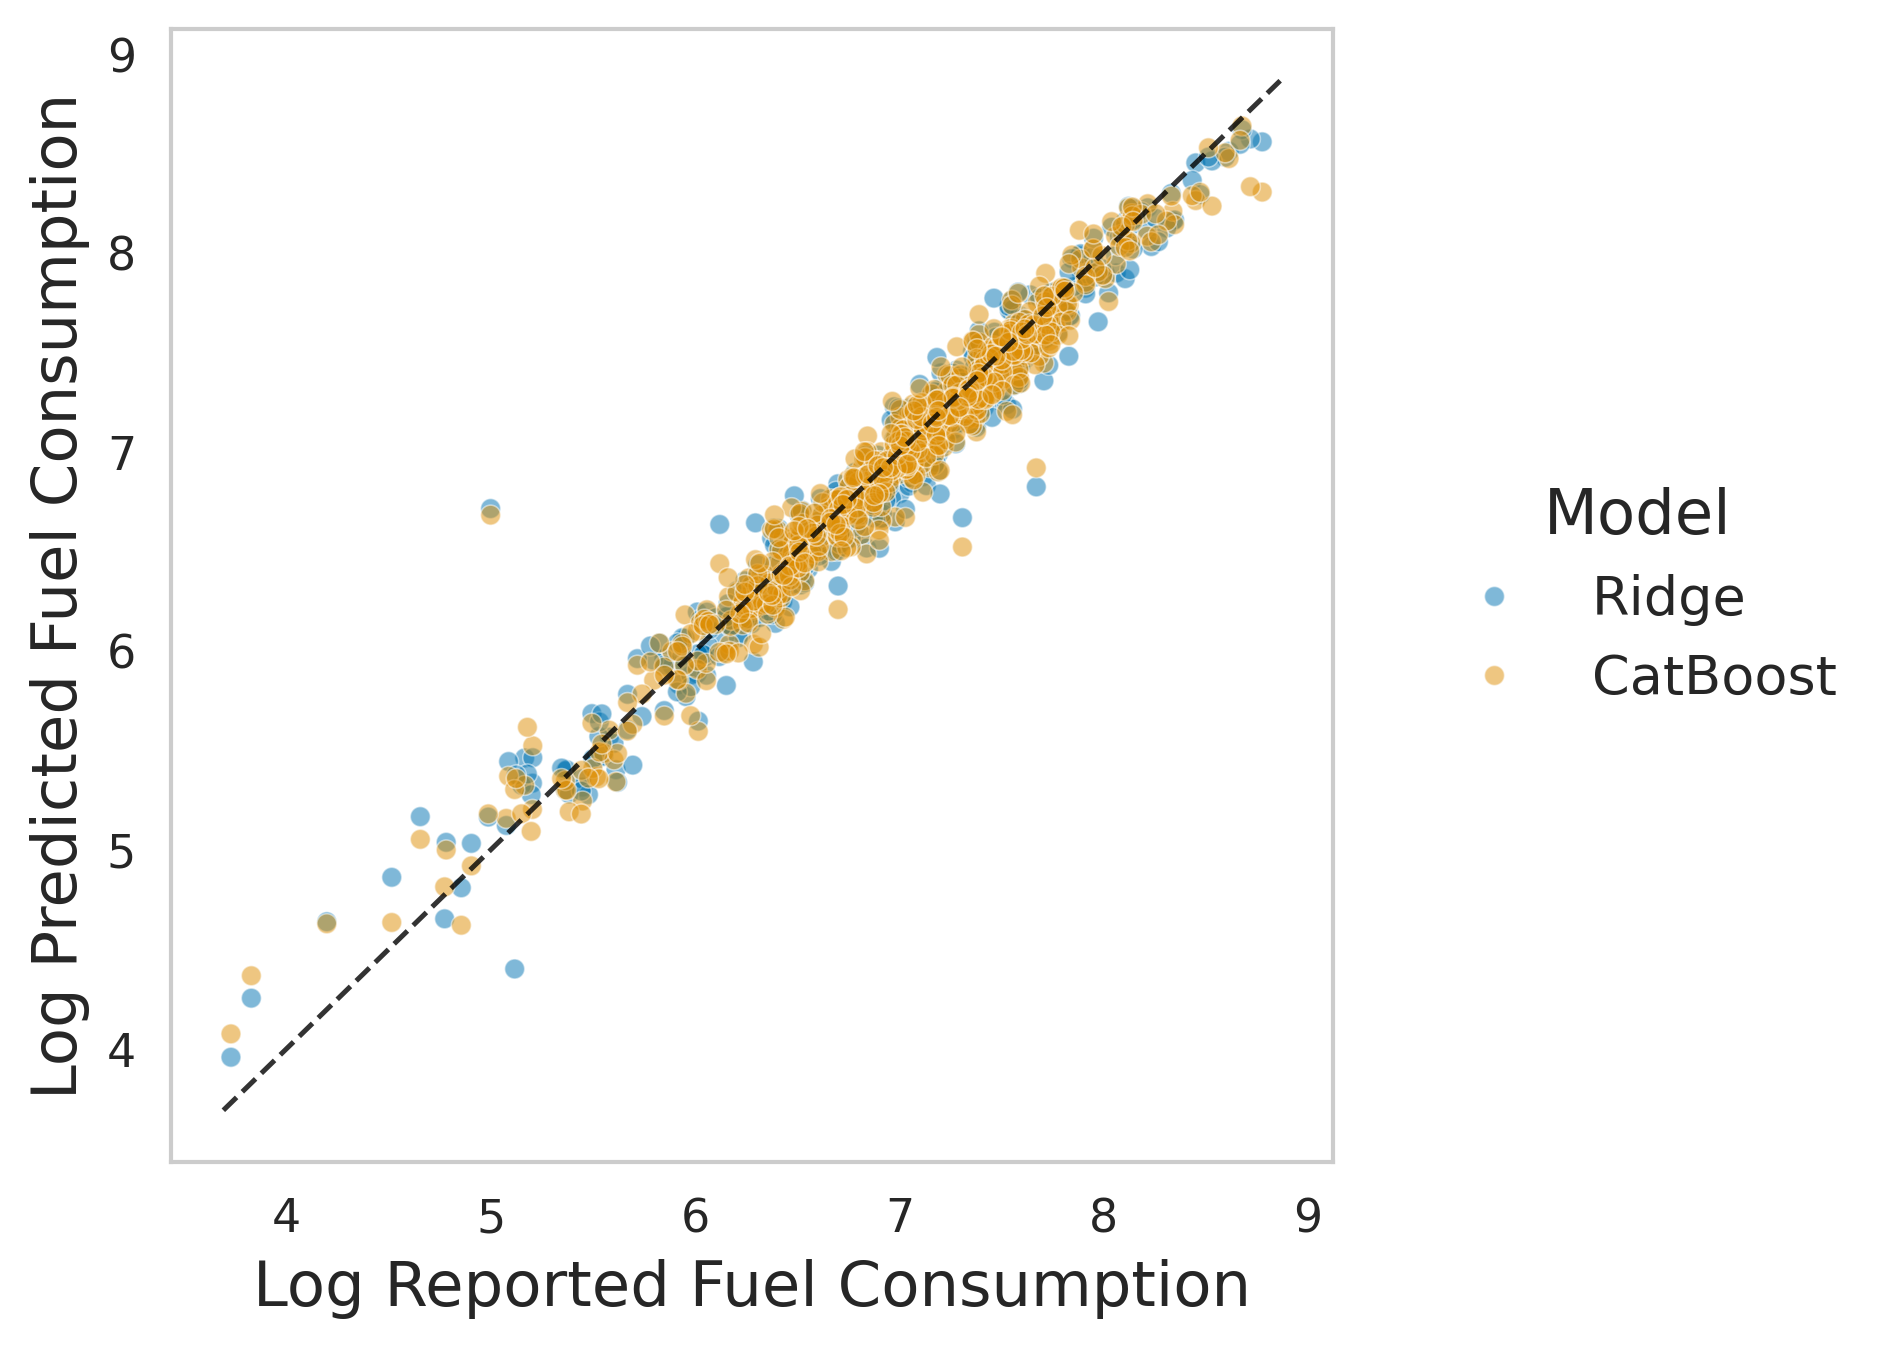
\includegraphics[width=0.65\textwidth]{ML_FC_Fm5dd_twoway_test_logs_compare2.png}
    \caption{Test set prediction accuracy (log-log) for ridge regression and CatBoost}
    \label{fig:twoway_test_compare2}
\end{figure}

% TODO: Discuss error-handling capacity of estimation over calculation

% TODO: Linear vs. non-linear models
% Why do some models work better than others?
% discuss log-additive discrepancy
% use feature importance to explain this
% is taking logs why linear models work so well?

% TODO: Feature importance
% TODO: dicuss utility of error variables and others
% for best? doesn't account for collinearity
% by groups? just run different subsets?

% Robustness
% - different feature sets?